\documentclass{IEEEtran}

\usepackage{mathtools}
\usepackage{amsmath}
\usepackage{graphicx}
\usepackage{subfig}
\usepackage{verbatim}
\usepackage{algpseudocode}
\usepackage{natbib}
\usepackage{url}
\usepackage{listings}
\usepackage[spanish]{babel}
\usepackage[utf8x]{inputenc}
\usepackage{float}
\usepackage{array}
\usepackage{booktabs}
%\setcounter{MaxMatrixCols}{16}

\begin{document}

\title{Informe Quizz 09}
\date {Mayo de 2013}
\author{\IEEEauthorblockN{Tatiana Lopez Guevara \\}
\IEEEauthorblockA{Universidad Tecnológica de Pereira\\
tatiana@sirius.utp.edu.co }}
\maketitle


\begin{abstract}
El presente documento explica los resultados obtenidos en la implementación del algoritmo
de RANSAC sobre un modelo lineal. La implementación se realizó sobre MATLAB.
\end{abstract}

\begin{IEEEkeywords}
Computer Vision
\end{IEEEkeywords}

\section{Introducción}
El modelo que explica los datos dados por el experimento físico es:

\begin{equation}
\begin{aligned}
y = a + b * \sin(x/10) + c*\sin(x/20)
\end{aligned}
\end{equation} 

El objetivo es entonces, estimar un modelo que no se vea afectado por los outliers
mediante el algoritmo de RANSAC.

Se tomó un valor de $n$ (tamaño de la muestra para estimar el modelo)
con un valor de 5 ya que se trata de un modelo lineal. La función
encargada de extraer este tamaño de muestra de los datos se encuentra
en el archivo \verb+random_sample.m+.

Con respecto al valor de $p$ (probabilidad de que al menos un conjunto de
$n$ datos tomados al azar no contenga outliers), se escogió en un valor
de $99\%$

Para la condición de salida $M$, se estableció un valor de 
$M = (1-\epsilon_0)n_{tot}$, donde para el valor de $\epsilon_0$
se tomó un valor de 0.25 cercano al recomendado en \cite{hartley2000multiple}.

El archivo principal de ejecución de esta tarea es \verb+runransac.m+.

\section{Ajuste del Modelo}
Para el ajuste del modelo se aplicó el método de mínimos cuadrados lineales 
(\textit{Linear Least Squares}) \cite{lls}.
El vector de $\vec{X}$ es una matriz de $Z$ x $3$, donde $Z$ es el número de observaciones
del modelo y las 3 columnas corresponden a los coeficientes de los parámetros de $\beta$.
La ecuación que se desea resolver, está dada por $\vec{X}\vec{\beta}=\vec{Y}$, donde:

\begin{equation*}
\begin{aligned}
\vec{X} = 
\begin{pmatrix}
1 & \sin(x_1/10) & \sin(x_1/20) \\ 
1 & \sin(x_2/10) & \sin(x_2/20) \\ 
\cdots & \cdots &  \cdots \\
1 & \sin(x_Z/10) & \sin(x_Z/20) \\ 
 \end{pmatrix} \\
\end{aligned}
\end{equation*} 
\begin{equation*}
\begin{aligned}
\vec{\beta} = \left(
\begin{array}{c}
a \\ 
b \\
c \\
 \end{array}
 \right) 
\end{aligned}
\end{equation*} 
\begin{equation*}
\begin{aligned}
 y =
\left(
\begin{array}{c}
y_1 \\ 
y_2 \\
\cdots \\
y_Z 
 \end{array}
 \right) 
\end{aligned}
\end{equation*} 

La solución a esta ecuación para el vector $\vec{\beta}$ está dada por:

\begin{equation*}
\begin{aligned}
\vec{\beta} = (\vec{X}^T \vec{X})^{-1} \vec{X}^T \vec{Y}
\end{aligned}
\end{equation*} 

El archivo \verb+get_model.m+ contiene la función encargada de realizar dicha
estimación.

\section{Concenso}

Una vez estimado el modelo con los datos de la muestra,
se procedió a umbralizar la distancia algebráica
con el modelo:

\begin{equation*}
\begin{aligned}
\vec{Y} - \vec{X}*\vec{\beta} = \epsilon \\
|\epsilon| < \delta
\end{aligned}
\end{equation*} 

Para obtener el concenso se asumió una dispersión del ruido
de $\sigma = 0.05$ con media 0. 
Un dato se consideró como \textit{outlier} si
está más lejos que 3 desviaciones estándar $3\sigma$.

La función en \verb+calc_si.m+ es la encargada de realizar
este proceso.

\section{Gráficas del Modelo}

En la gráfica \ref{fig:outliers} se muestra el resultado
obtenido mediante RANSAC en rojo contra el modelo real
y el modelo hallado mediante \textit{Linear Least Squares}
sobre todos los datos teniendo en cuenta los
\textit{outliers}. En esta última se ve que el modelo
es afectado por estos datos atípicos.

\begin{figure}[H]
\caption{Gráfica de Observaciones vs Modelo Real (azul), Modelo
obtenido con RANSAC + outliers (rojo), Modelo obtenido con LLS
sobre todos los datos incluyendo outliers (amarillo)}
\centering
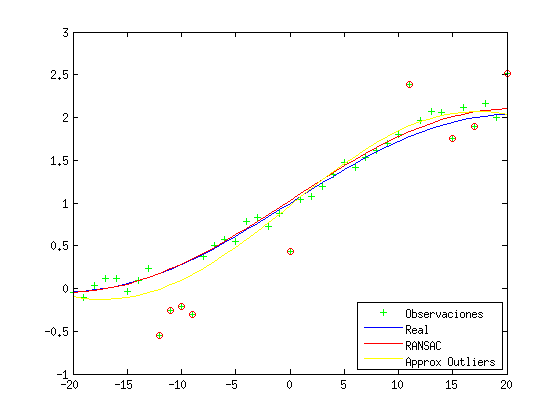
\includegraphics[width=9.5cm,natwidth=560,natheight=420]{figs/outliers.png}
\label{fig:outliers}
\end{figure}

\section{Root Mean Square Error - RMSE}
Se obtuvo un Error RMSE = 0.001410 después
de ejecutar N=1000 simulaciones de Monte Carlo.

\begin{equation*}
\begin{aligned}
RMSE = \sqrt \frac{1}{n_{tot}} \displaystyle\sum_{i=1}^{n_{tot}} (\vec{Y} - \vec{X}\vec{\beta})^2
\end{aligned}
\end{equation*} 

\section{Conclusiones}
\begin{itemize}
\item El algoritmo de RANSAC converge de forma 
rápida (promedio de 14 iteraciones)
comparado con el total de posibilidades
que se deberían evaluar mediante fuerza bruta
$\binom{41}{5} = 749398$.
\item El método de RANSAC presenta una aproximación
muy cercana al modelo real, aunque hay que asumir
de antemano que los errores tienen alguna desviación
estándar y tienen media 0.
\item De igual forma, para la variable $M$ que indica
una de las condiciones de salida del algoritmo exige
asumir una probabilidad de outliers que de antemano
es difícil conocer en otra situación. En este modelo
fue fácil ya que se tenían a disposición todos los datos
del sistema.
\end{itemize} 

\bibliographystyle{plain}
\bibliography{biblio}

\end{document}
